\documentclass[letterpaper, 12pt]{article}


\usepackage{parskip,xspace}
\usepackage{amsmath,amsthm,amsfonts,amssymb}
\usepackage{mathrsfs} 
\usepackage{caption}
\usepackage{xcolor} 
\usepackage{geometry}
\usepackage{fancyhdr}
\usepackage{rotating}
\usepackage{multirow}
\usepackage{makecell}
\usepackage{ltxtable}
\usepackage{hyperref}
\usepackage{graphicx}
\usepackage{subfigure}
\usepackage{bm}
\usepackage[]{statrep}
\usepackage{enumerate}
\usepackage{subfigure}
\usepackage[toc,page]{appendix}

\graphicspath{{eps/}}


\newcommand{\ba}{$$\begin{aligned}}
\newcommand{\ea}{\end{aligned}$$}
\newcommand{\dx}{\mathrm{d}x}
\newcommand{\lma}{\left(\begin{matrix}}
\newcommand{\rma}{\end{matrix}\right)}




\pagestyle{fancy}
\lhead{Peng Shao 14221765}
\chead{}
\rhead{\bfseries STAT 8320 Spring 2015 Assignment 6}
\renewcommand{\headrulewidth}{0.4 pt}
\setlength{\parindent}{2em}

\begin{document}
\title{STAT 8320 Spring 2015 Assignment 6}
\author{Peng Shao 14221765}
\maketitle
\indent




$\blacktriangleright$ \textbf{1.\quad Solution.} 
(a). Because PCA is not invariant with respect to changes in scale, that is, the variable which is measured under larger scale will have larger variance, then produce a large eigenvalue when performing singular value decomposition. So standardization avoids the problems of having one variable with large variance unduly influencing the determination of factor loadings, and the correlation matrix is the covariance matrix of standardized variable.

(b). Before PCA, we should investigate the data roughly, and we find that there may be an outlier which have the total score less than 6000. We have no idea why cause this abnormality, but we should take it out of the following analysis because the PCA is very sensitive to outliers. Then we do a PCA based on the 10 single scores.

\begin{figure}[htbp]
\centering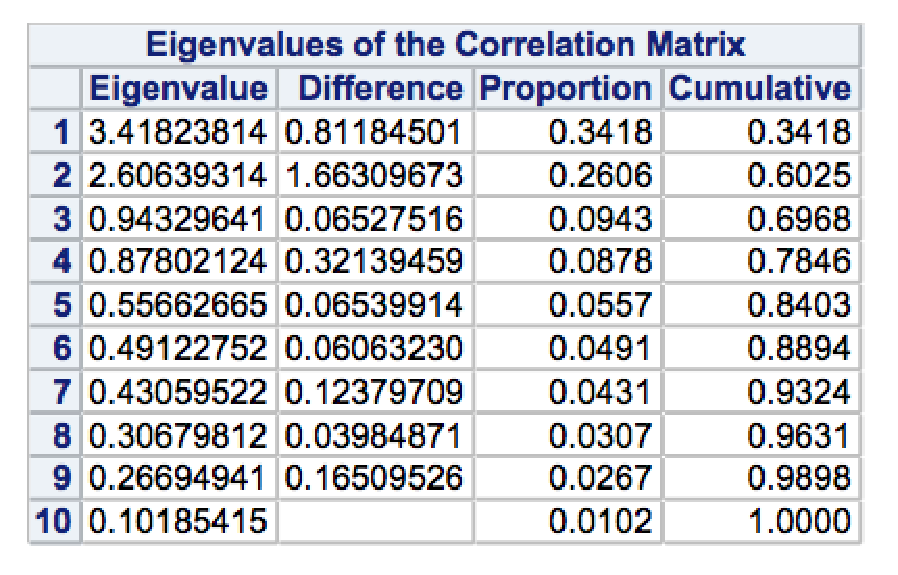
\includegraphics[width=3.5in]{7-1.eps}
\caption{Principal Component Proportion}\label{1}
\end{figure}

From Figure \ref{1}, the first 2 PCs have accounted for 65.25\% variability of the total.


(c).
Because the first 2 PCs account for more than 50\% variability of the data, and the only these 2 PCs have the eigenvalues more than 1.

(d). 
\begin{figure}[htbp]
\centering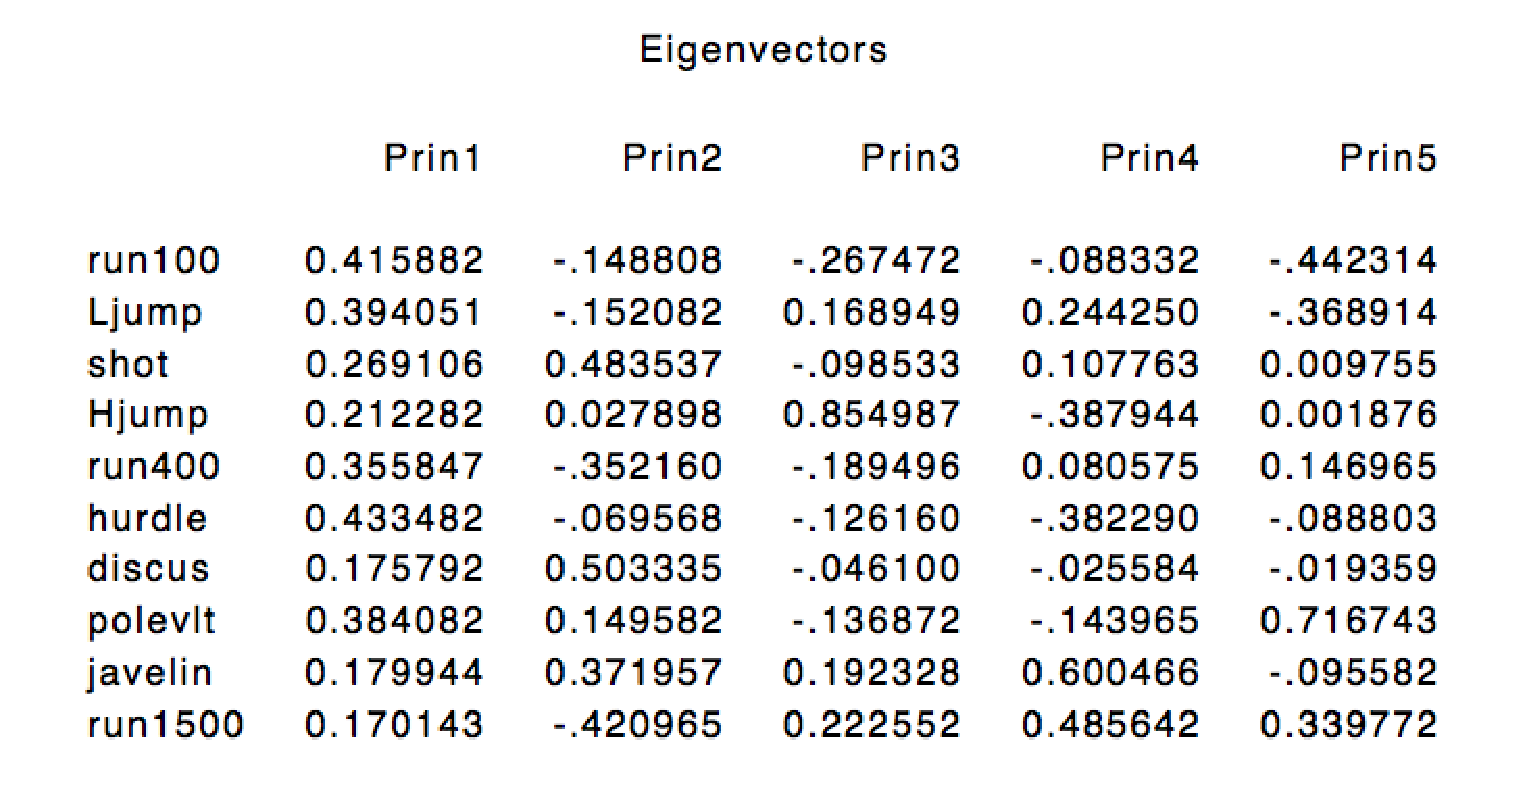
\includegraphics[width=5in]{7-2.eps}
\caption{First 5 Principal Components}\label{2}
\end{figure}
According to the part of PC table (Figure \ref{2}), the first principal component may be a kind of overall means of all scores, not exactly equal to the average because of some slightly different weights; and the second principal component may be the comparison between the scores of running add long jump and those of throwing add pole vault. 


(e). \begin{figure}[htbp]
\centering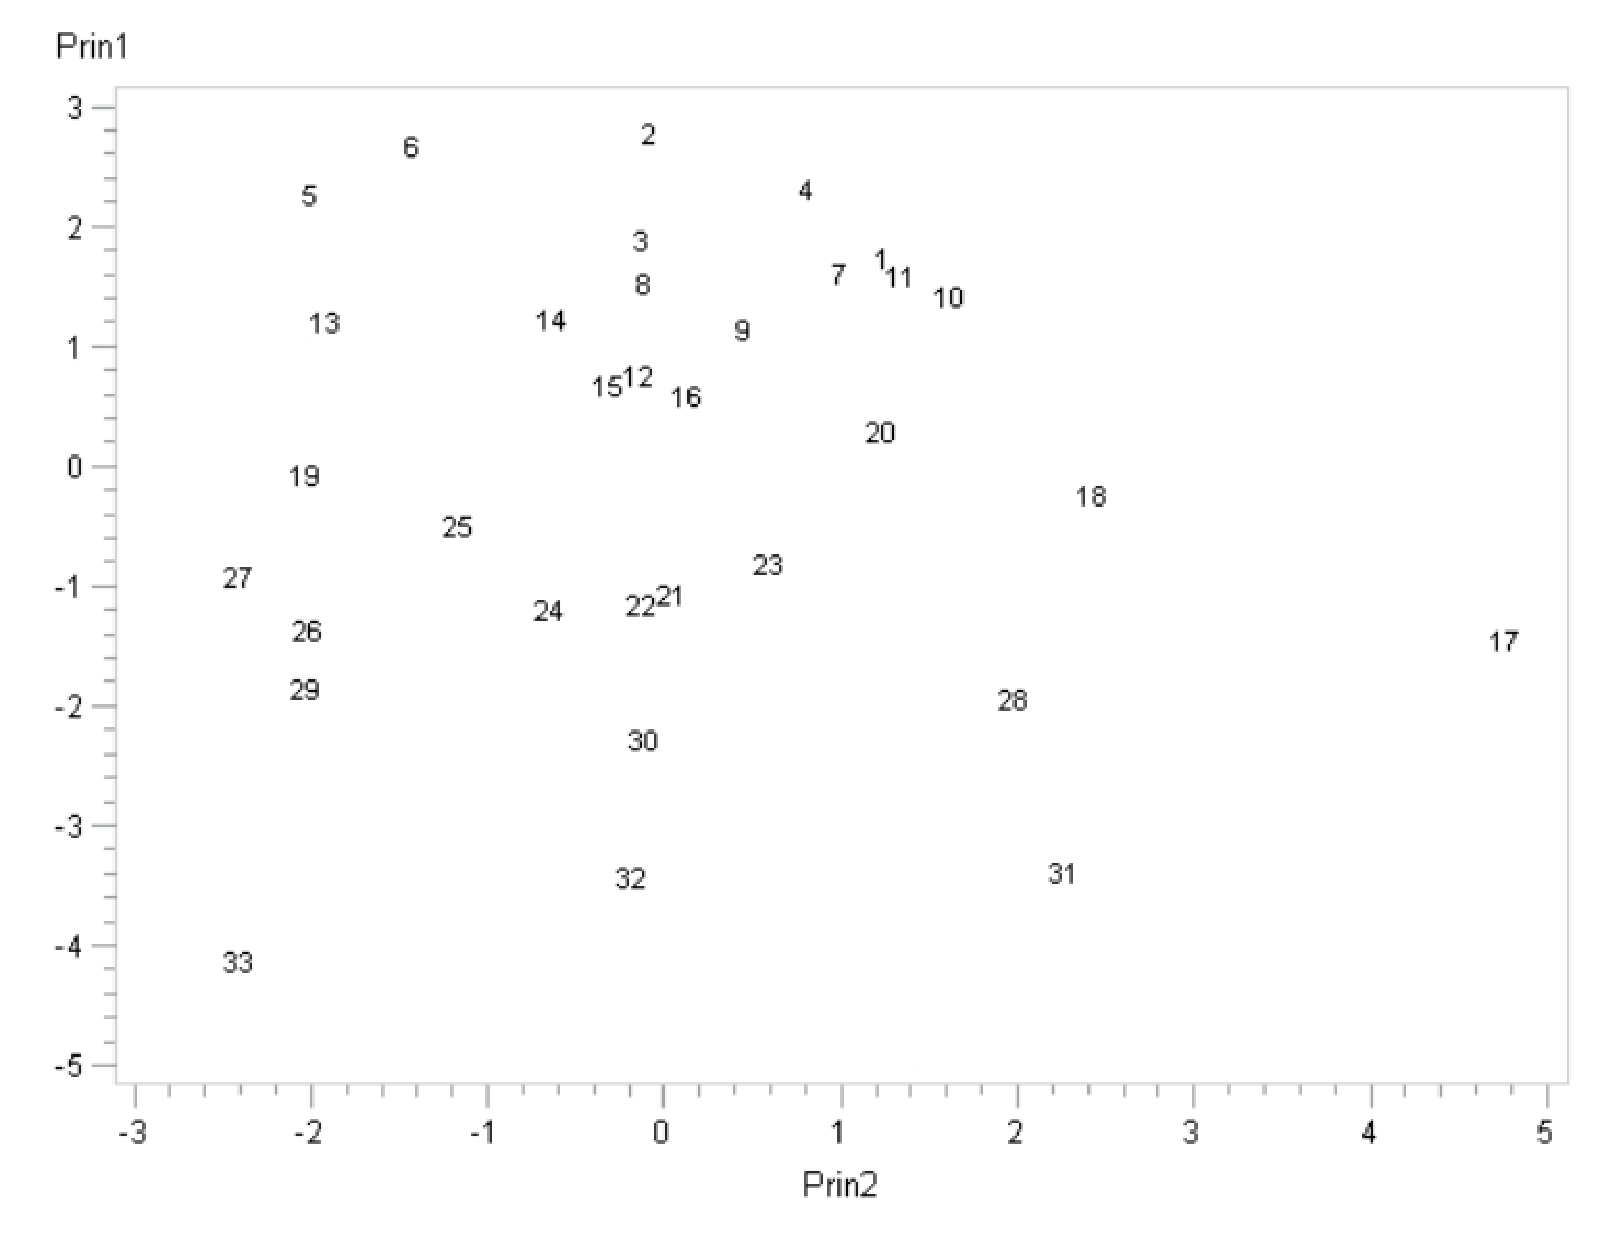
\includegraphics[width=5in]{7-3.eps}
\caption{1st PC v.s. 2nd PC}\label{3}
\end{figure}

From the scatter plot Figure \ref{3}, the data points have already been labeled as the their rank. So we can see that most high rank athletes (here higher rank means higher total score but smaller value of the rank) have comparably high 1st PC score. However, it is hard to see that whether there is any pattern of 2nd PC score relative to the ranks of athletes. 

Hence, to make the relationship between PC scores and the ranks (or the total scores) more clearly, we can plot the total score versus two PC scores respectively(Figure \ref{4} and Figure \ref{5}). From Figure \ref{4}, we can see that the 1st PC score has positive relationship with total score indeed, and we also believe that there should be no significant relationship between 2nd PC score and total score.
\begin{figure}[htbp]
\begin{minipage}[t]{0.5\linewidth}
\centering
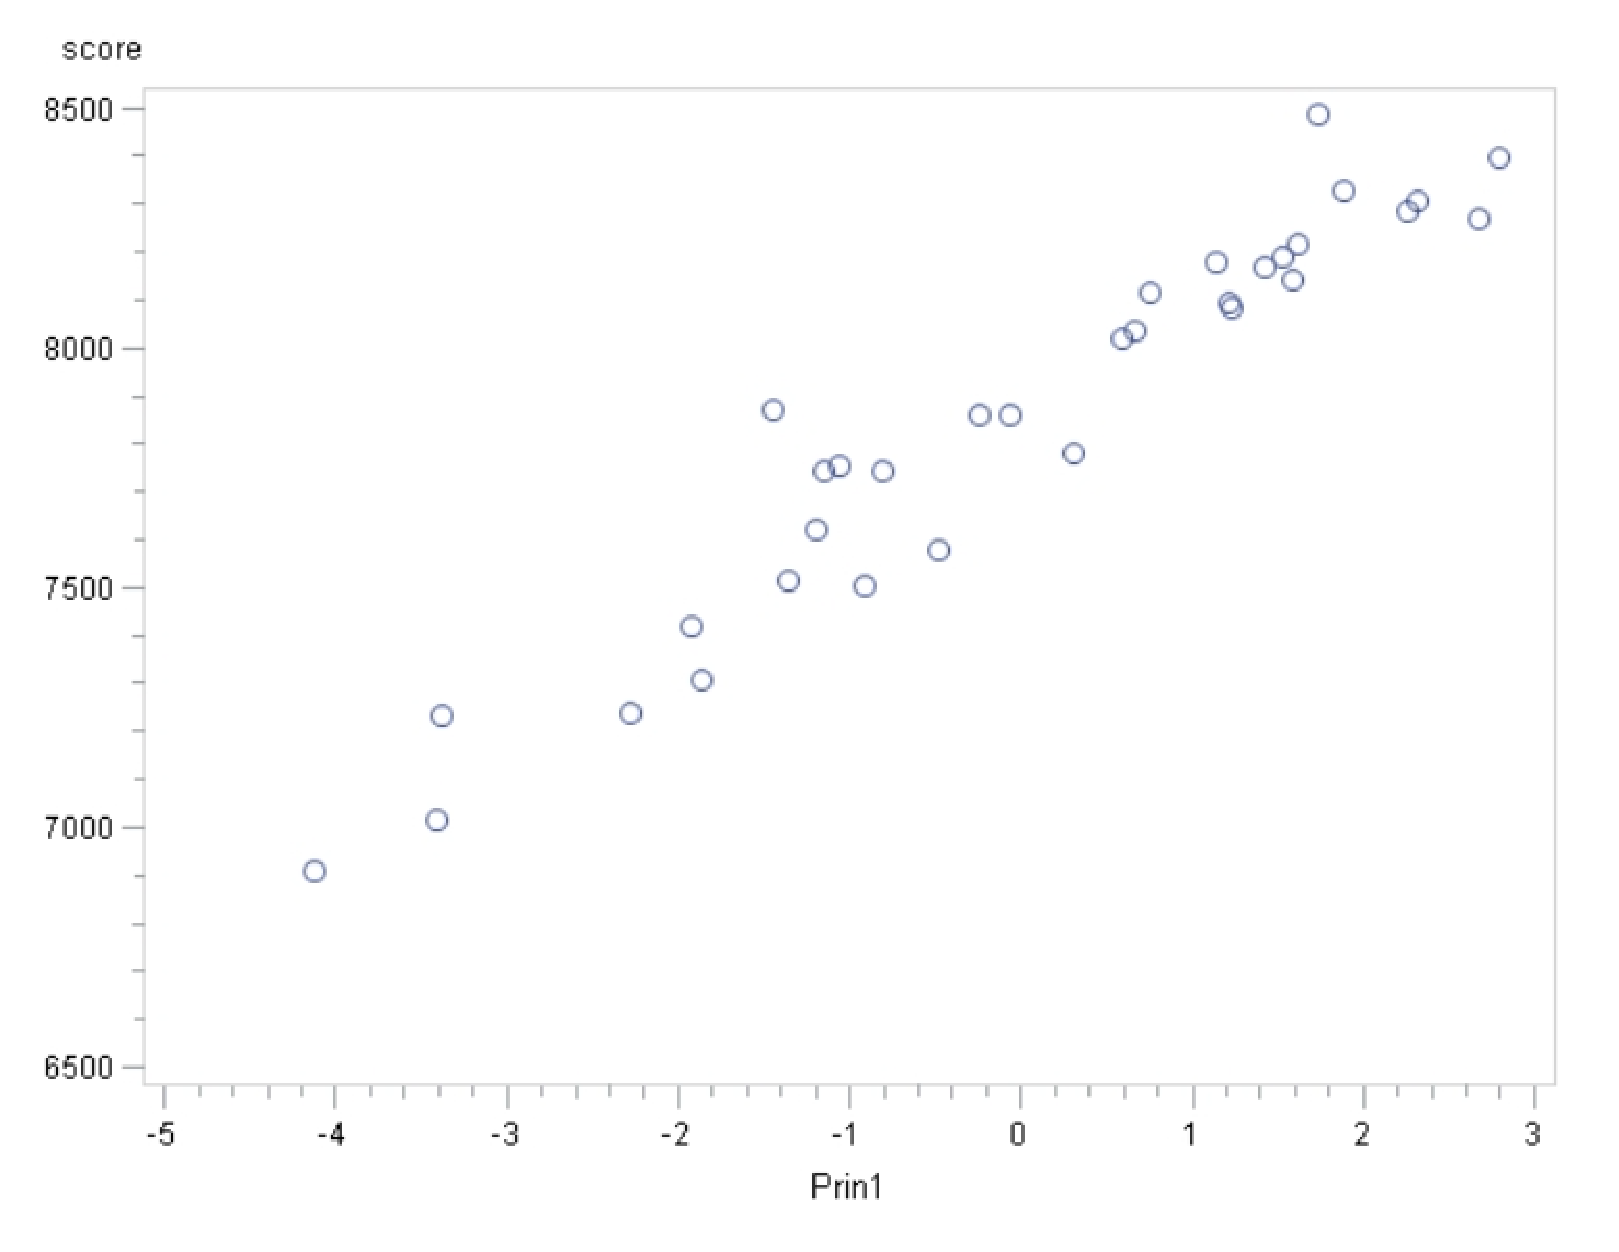
\includegraphics[width=3in]{7-4.eps}
\caption{Total Score v.s. 1st PC}\label{4}
\end{minipage}
\begin{minipage}[t]{0.5\linewidth}
\centering
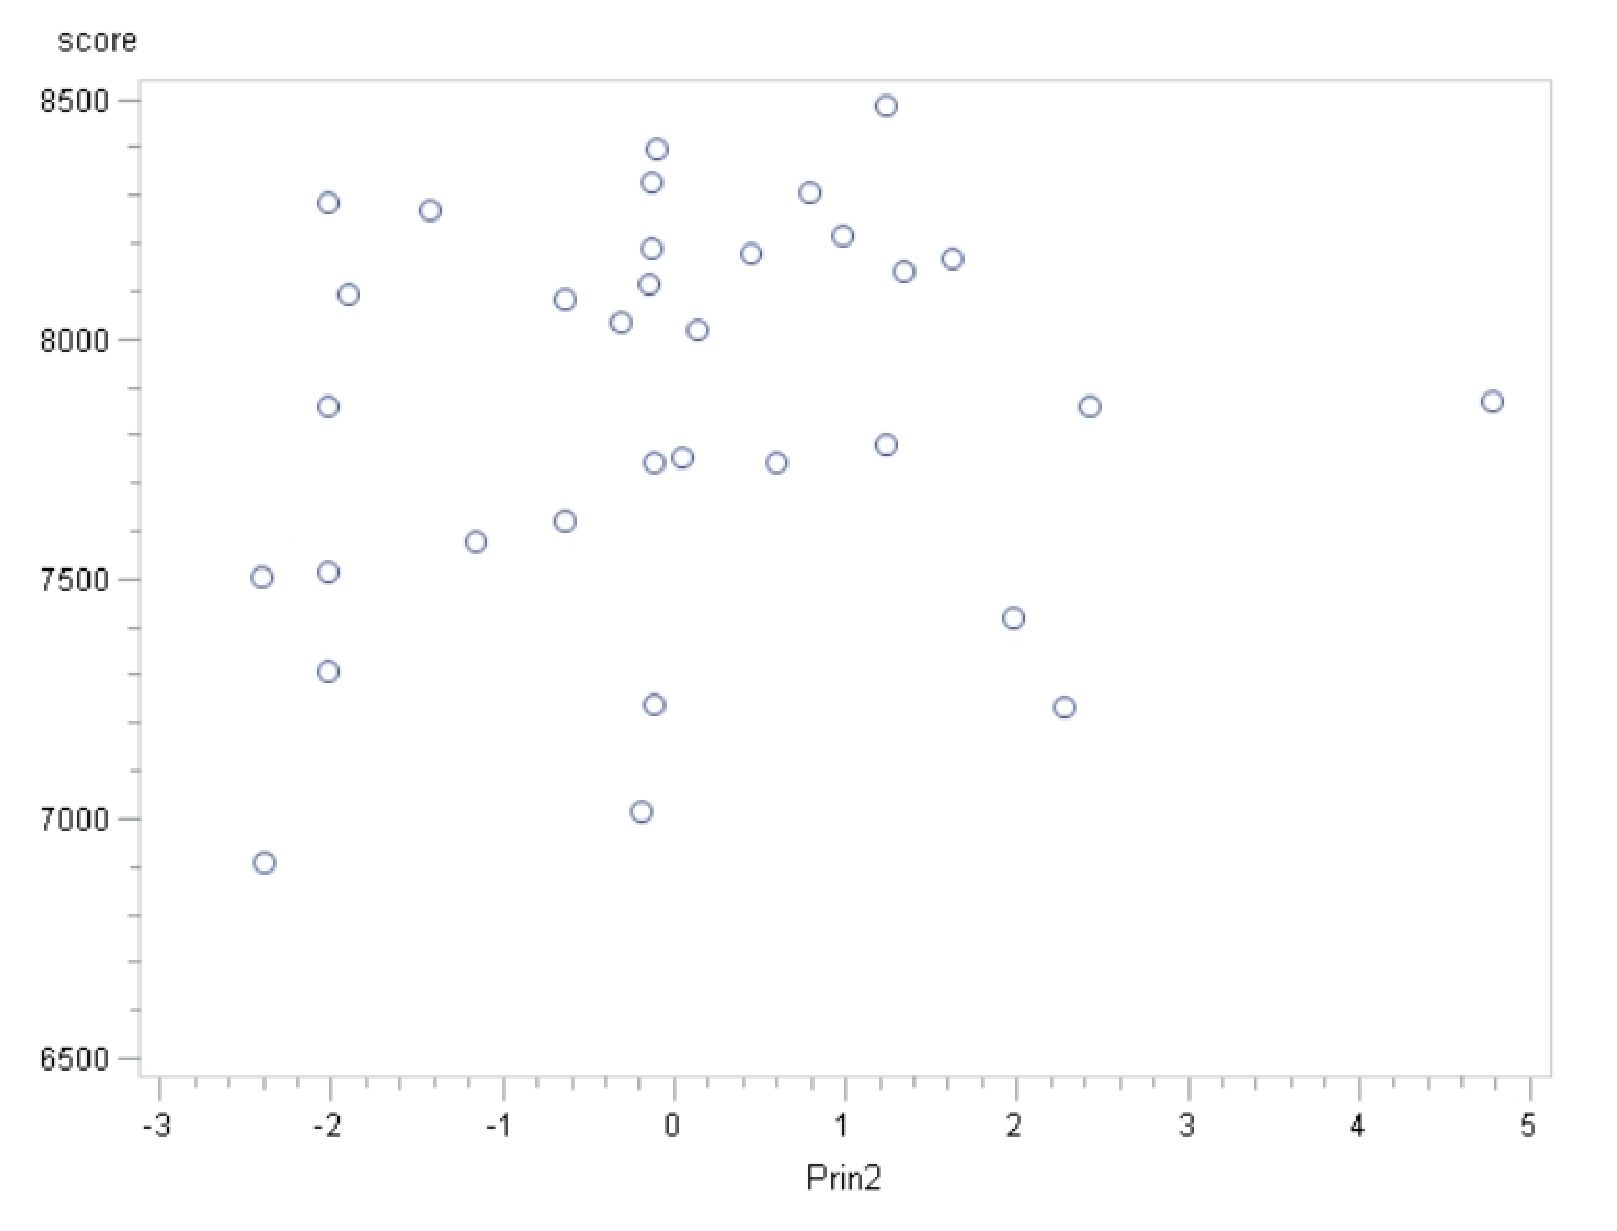
\includegraphics[width=3in]{7-5.eps}
\caption{Total Score v.s. 2nd PC}\label{5}
\end{minipage}
\end{figure}


(f). \begin{figure}[htbp]
\centering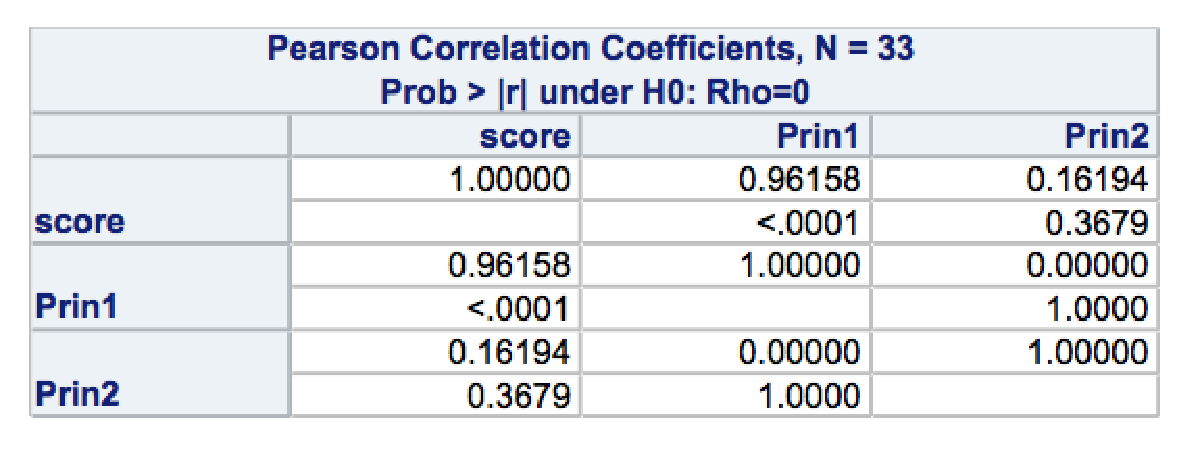
\includegraphics[width=4in]{77.eps}
\caption{Correlation Matrix among PCs}
\end{figure}

To compute the Pearson correlation coefficients among the total score, 1st PC score and 2nd PC score. The correlation coefficient between total score and 1st PC score is 0.96158 while that between total score and 2nd PC score is only 0.16194. This is in accordance with the result of last part. Thus, we may guess that the total score should be measured in a way like 1st PC, i.e., a kind of overall mean, not some comparisons.




$\blacktriangleright$ \textbf{2.\quad Solution.} 
(a). Because $X_i$ are standardized random variables(zero mean and one standard deviation), then the covariance of $X_i$ is exactly the correlation of $X_i$. So
\ba
corr(X_i,X_k)&=cov(X_i,X_k)=cov(a_iF+e_i,a_kF+e_K)\\
&=a_ia_kvar(F)+a_icov(F,e_k)+a_kcov(e_i,F)+cov(e_i,e_k)=a_ia_k\\
corr(X_j,X_k)&=cov(X_j,X_k)=cov(a_jF+e_j,a_kF+e_K)\\
&=a_ja_kvar(F)+a_jcov(F,e_k)+a_kcov(e_j,F)+cov(e_j,e_k)=a_ja_k\\
\ea
where $i,j,k$ are mutually different. Thus the ratio of pair of rows $(i,j)$ is always
$$
\frac{corr(X_i,X_k)}{corr(X_j,X_k)}=\frac{a_i}{a_j}
$$
for all $k\not=i,j$.


(b). 
$$
corr(\bm{X})=\lma a_1\\a_2\\a_3\\a_4\\a_5\\a_6\rma\lma a_1&a_2&a_3&a_4&a_5&a_6\rma+var(\bm{e})
$$

(c). 
$$
\bm{X}=\bm{a}F+\bm{e}
$$
where 
\begin{itemize}
\item $\bm{X}=\lma X_1&X_2&\cdots&X_6\rma'\sim \text{N}(\bm{0},corr(\bm{X}))$
\item $F\sim\text{N}(0,1)$
\item $\bm{a}=\lma a_1&a_2&\cdots&a_6\rma'$
\item $\bm{e}=\lma e_1&e_2&\cdots&e_6\rma'\sim \text{N}(\bm{0},\bm{\Psi})$
\item $F$ and $\bm{e}$ are independent.
\end{itemize}


(d). For my perspective, only one factor should be included. Because
\begin{enumerate}
\item only the eigenvalue of the 1st factor is larger than 1, no matter how many factor we include in the analysis, and the proportion of variability accounted by the 1st factor is at least 100\%.
\item to test the hypothesis
$$
H_0:\text{ 1 Factor is sufficient}
$$
the P-value is 0.9805, so we cannot reject the null hypothesis, that is, more factors are not necessary.
\item the AIC and BIC of one factor are lower than those of two factors.
\end{enumerate}

(e). The result of "Factor Pattern" can give the information about factor loadings of different variable, i.e. the $a_i$ in the model in part (c). For example, the variable C has a loading of 0.95611(a very high loading) in Factor1, and the variable F has a loading of 0.87081(a moderately to high loading) in Factor1, and so on. All variables have a at least moderately to high loading in Factor1, and the loadings are not different so much.

In addition, we can know how much proportion of variance of each variable is accounted by the communality from the "Factor Pattern" output or "Final Communality" output. For example, 
$$
\text{Communality of C}=a_1^2=0.95611^2=0.9141
$$
which means 91.41\% variability of C comes from common factor and only 8.69\% variability come from specific factor.

(f). No. If the rotation is help, let $T$ become the rotation operator. Then we can have that
$$
F^*=TF
$$
where the $F^*$ is the factor after rotating. So the $F^*$ should also have the restriction of length equal to 1, i.e. $var(F^*)=1$. This implies that $T^2=1$, and so $T=\pm1$. So rotation cannot change the value of loadings except the sign. Thus, there is no need to perform a rotation.


(g). Because we choose to include only one factor in the model and the loadings and communality are high comparing to specific factor. That is to say, all variable perform like the only one common factor, so they should perform similarly to each other. Then the correlations between them should looks same.








$\blacktriangleright$ \textbf{3.\quad Solution.} 
(a). \begin{figure}[htbp]
\centering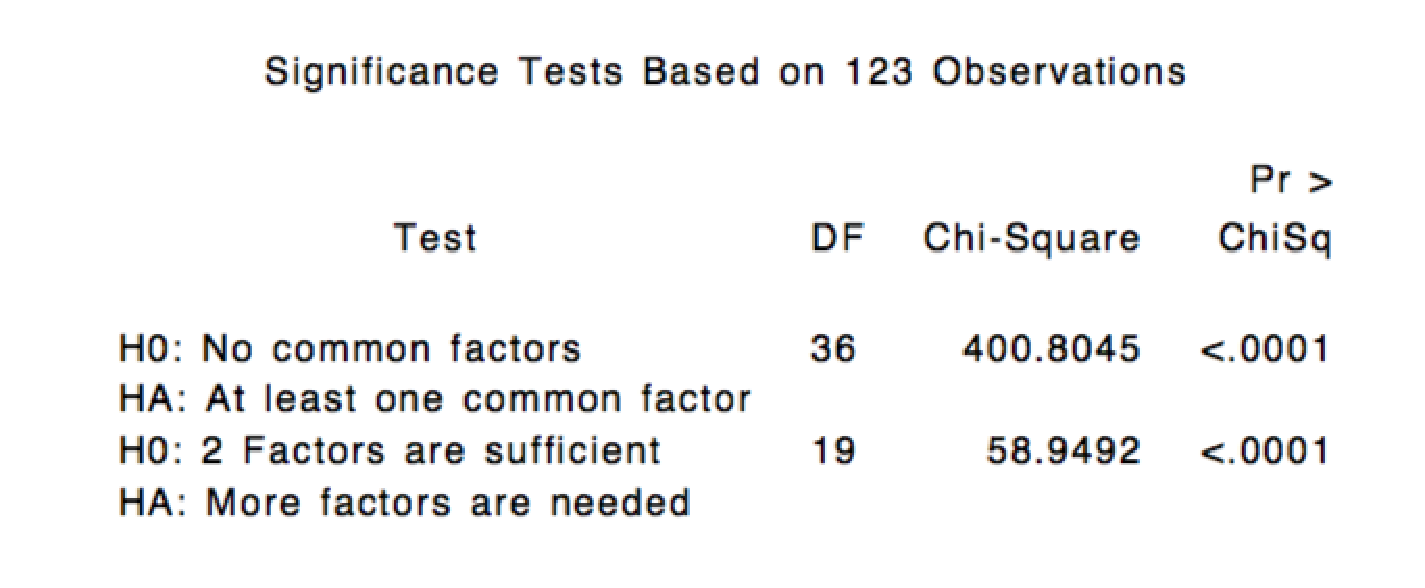
\includegraphics[width=4in]{7-6.eps}
\caption{Likelihood Tests}\label{6}
\end{figure}

No. From the second test in Figure \ref{6}, the P-value less than 0.0001 means we should reject the null hypothesis, that is, two factors is not sufficient.

(b). \begin{figure}[htbp]
\centering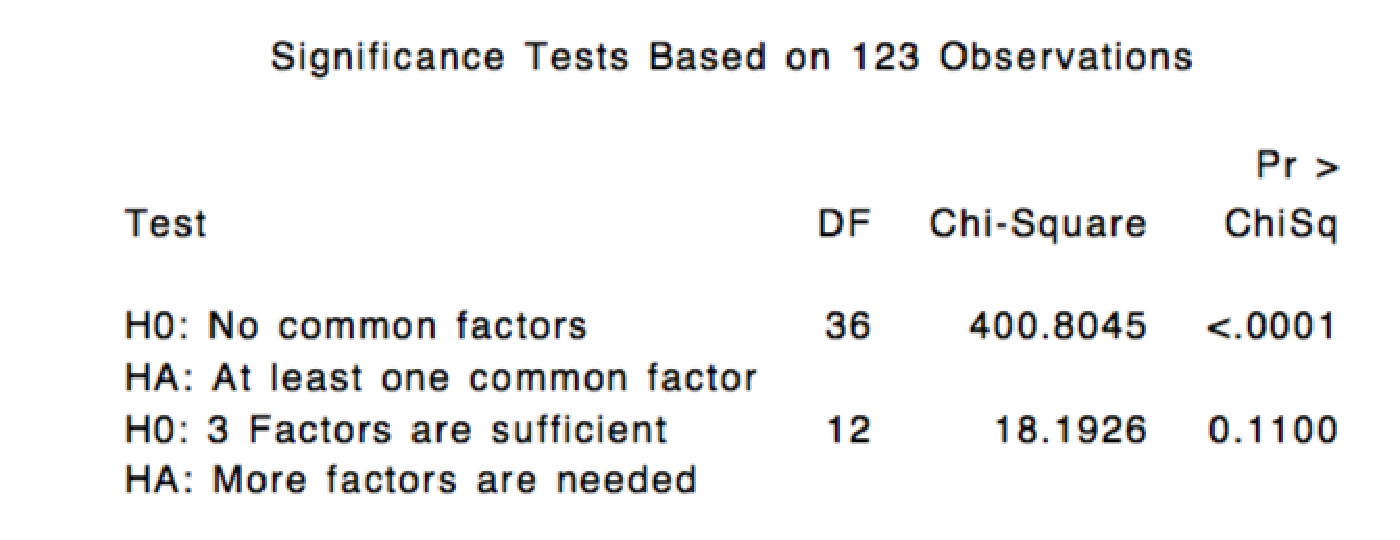
\includegraphics[width=4in]{7-7.eps}
\caption{Likelihood Tests}\label{7}
\end{figure}
Yes. From the second test in Figure \ref{7}, the P-value=0.1100 means we do not reject the null hypothesis, that is, 3 factors is sufficient.

\begin{figure}[htbp]
\centering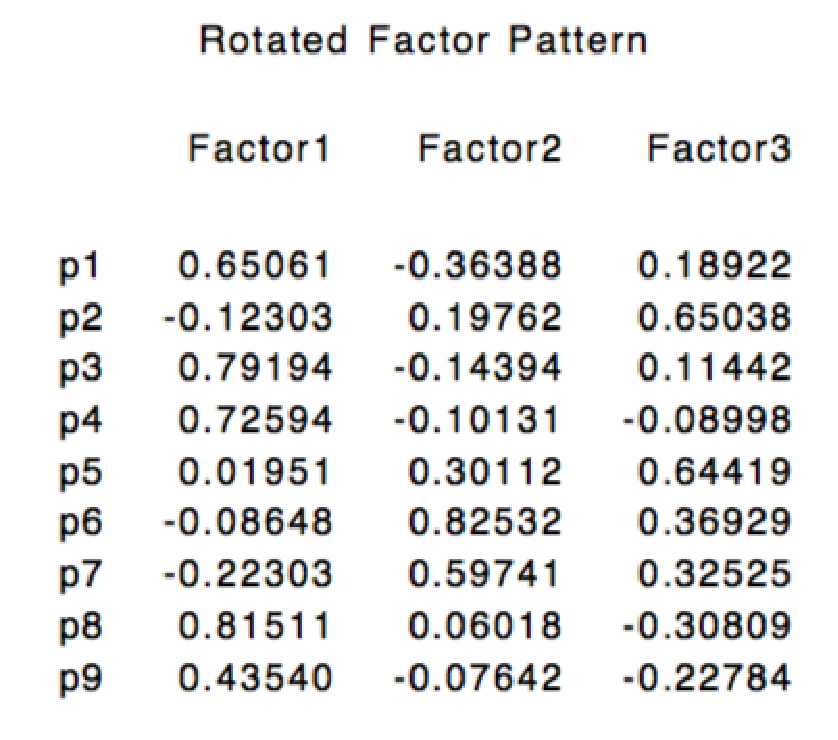
\includegraphics[width=3in]{7-8.eps}
\caption{Rotated Factors}\label{8}
\end{figure}
From the Figure \ref{8}, we can see that $p1,p3,p4,p8,p9$ have high loadings in factor 1, and all there statements have mentioned doctor. So maybe the factor 1 is a "doctor factor". $p6,p7$ have high loadings in factor 2, and all these statements is about themselves without some specific reasons. So maybe the factor 2 is a "subjective personal factor". $p2,p5$ have high loadings in factor 3, and all these statements is also about themselves but more reasonable. So maybe the factor 3 is a "objective personal factor".


(c). \begin{figure}[htbp]
\centering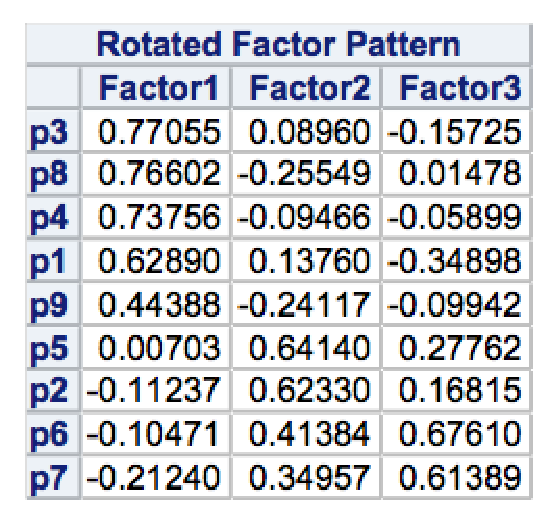
\includegraphics[width=2.5in]{7-9.eps}
\caption{Rotated Factors}\label{9}
\end{figure}
From the Figure \ref{9}, we can see that the factor pattern does not change too much between MLE and principle factor method; the clusters are still same: $\{p3,p8,p4,p1,p9\},\{p5,p2\},\{p6,p7\}$, only the loadings change slightly. But the interpretation becomes a little different. Because principle factor method uses the philosophy of PCA, so the factor interpretation may be like the interpretation of PCs. That is, factor 1 is the overall mean of $\{p3,p8,p4,p1,p9\}$, factor 2 is the overall mean of $\{p5,p2\}$ and factor 3 is the overall mean of $\{p6,p7\}$.


(d). \begin{figure}[htbp]
\centering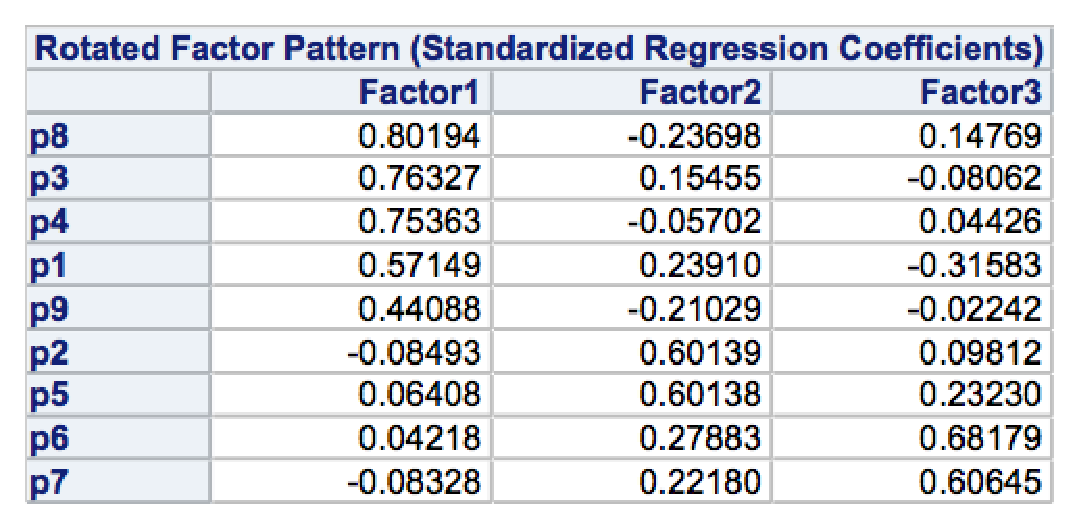
\includegraphics[width=4in]{7-10.eps}
\caption{Oblique Rotated Factors}\label{10}
\end{figure}
The overall result of principle factor method with oblique rotation is not so different from the result of other methods. It also only has some differences about factor loadings. The clusters and the interpretations of factors are same as the principle factor method with orthogonal rotation. However, for oblique rotation, we should also see the correlation between latent factors. In the problem the maximum correlation coefficient is 0.33129, which is not significant. So we can stop here. If the correlation between factors is significant, we can go on and perform a factor analysis to get the second order factor, which may contain more general information.



\end{document}
